\documentclass{book}
\usepackage{graphicx}
\usepackage{amsmath}
\usepackage{amsfonts}
\usepackage{musicography}

\newtheorem{definition}{Definition}
\newcommand{\muskern}{\kern-.15ex }
\makeatletter
\newcommand\dynmark[1]{{\normalfont\bfseries\itshape
  \@tfor\next:=#1\do{\put@muskern\next}\/}}
\newcommand{\put@muskern}{\let\put@muskern\muskern}
\makeatother

\begin{document}
    \chapter{Fundamentals}
    \section{Pitch}
\begin{definition}[Pitch]
    Pitch is the property of the sound which allows a relative ordering of perceived sounds on a frequency-related scale.
\end{definition}
On a keyboard, pitch goes up to the right of the keyboard, while it goes down on the left.

Pitches are expressed through \textbf{notes}. There are 7 note names\footnote{C-B in anglophone countries, C-H in Germany and Do-Si for the rest of Europe.}, which are repeated in \textbf{octave registers}, identified by the bottom number.
$$\cdots A_3 B_3 \underbrace{C_4 D_4 E_4 F_4 G_4 A_4 B_4}_{\text{Octave register 4}} C_5 D_5 \cdots$$

\begin{figure}[h]
    \begin{center}
        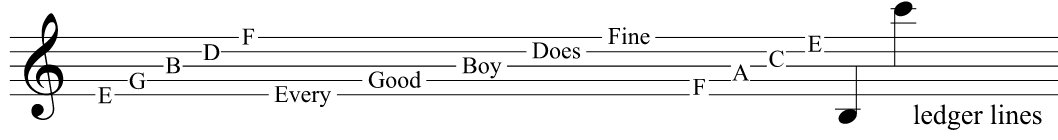
\includegraphics[width=0.8\textwidth]{img/treble}
        \caption{Treble clef}
        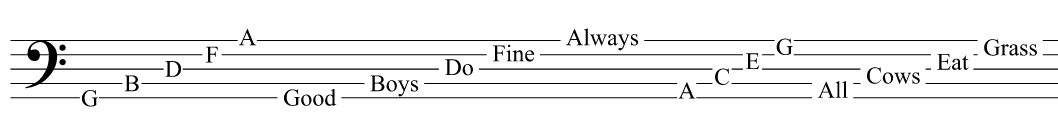
\includegraphics[width=0.8\textwidth]{img/bass}
        \caption{Bass clef}
    \end{center}
\end{figure}

\begin{definition}[Octave]
    The distance / interval between two notes with the same name.
\end{definition}

\begin{definition}[Middle C]
    The $C_4$ pitch, usually located in the middle of a keyboard (on the instrument) and always annotated in the middle of the grand staff, shared by the two staves.
\end{definition}

\begin{figure}[t]
    \begin{center}
        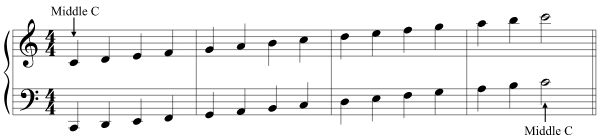
\includegraphics[width=0.8\textwidth]{img/grandstaff}
        \caption{The Grand Staff (a specific stave \emph{system})}
    \end{center}
\end{figure}

\begin{definition}[Accidental]
    A symbol placed before a note to raise / lower its pitch by a given amount.
\end{definition}

An accidental is effective only for a measure. They affect the entire piece if they are placed before the clef in a \textbf{key signature}.
\begin{center}
    \begin{tabular}{r|c|l}
        $\flat{}$ & Flat & $-1$ half step \\
        $\sharp{}$ & Sharp & $+1$ half step \\
        $\musDoubleFlat$ & Double flat & $-2$ half steps / $-1$ whole step \\
        $\musDoubleSharp$ & Double sharp & $+2$ half steps / $+1$ whole step \\
        $\natural{}$ & Natural & Cancels preceding accidentals \\
    \end{tabular}
\end{center}
There exists also \textbf{half-accidentals}, whose altered notes cannot be played on a keyboard.

\begin{definition}[Half step]
    On the keyboard, the distance / interval between one key (either black or white) and the next (either black or white).
\end{definition}

\begin{definition}[Whole step]
    The interval made up of two half steps.
\end{definition}

\begin{figure}[h]
    \begin{center}
        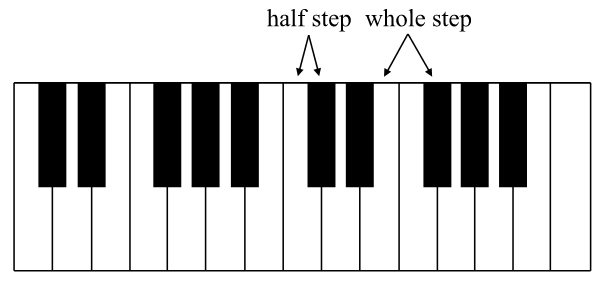
\includegraphics[width=0.6\textwidth]{img/halfstep}
        \caption{Half steps and whole steps}
    \end{center}
\end{figure}

\begin{definition}[Enharmonic]
    Which has the same sound, but different name.
\end{definition}

\section{Rhythm}
\begin{definition}[Beat / pulse]
    The basic pulse underlying measured music and thus the unit by which musical time is reckoned.
\end{definition}

\begin{definition}[Tempo]
    Speed of the beat.
\end{definition}
The tempo is usually expressed through metronome markings in \textbf{BPM / Beats Per Minute}.

\subsection{Time signatures}

\begin{figure}[h]
    \begin{center}
        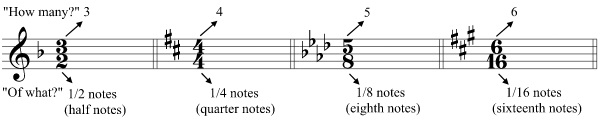
\includegraphics[width=1\textwidth]{img/timesignature}
        \caption{Meaning of the time signatures}
    \end{center}
\end{figure}

\subsection{Note / rests durations}
Both notes and rests last for certain duration, which is always a $2^n$ number of beats, where $n \in \mathbb Z$. Common values for $2^n$ are the following ones:

$$\left\{4,2,1,\frac{1}{2}, \frac{1}{4}\right\} \text{ beats}$$

Values different from these ones can be gathered through \textbf{ties} and \textbf{dots}. A dot adds $\frac{1}{2}$ the value of the note dotted, while a double dot adds $\frac{1}{2} + \frac{1}{4}$ the original value.

\subsection{Meters}
\begin{definition}[Meter]
    Describes the number of beats in a measure / bar and how they are divided.
\end{definition}

\textbf{Simple meters} break the beat into 2 parts, while \textbf{compound meters} break it into 3 parts.

They can be \textbf{double} (2 beats / bar), \textbf{triple} (3 beats / bar) or \textbf{quadruple} (4 beats / bar).

\begin{figure}[h]
    \begin{center}
        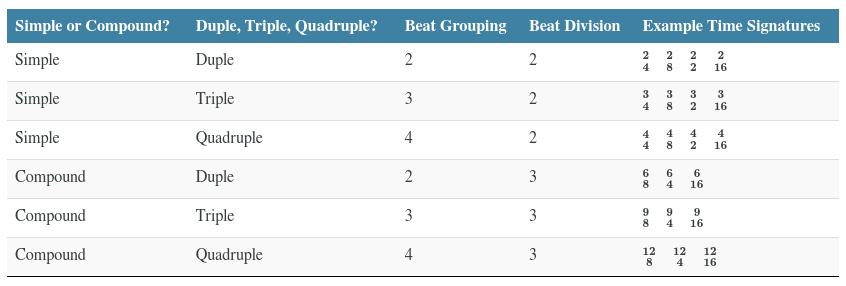
\includegraphics[width=1\textwidth]{img/meters}
        \caption{Meters}
    \end{center}
\end{figure}

The meter is traditionally identified by the time signature.

When a piece shifts between time signatures / meters often the composers employ a \textbf{metric modulation}.

\begin{definition}[Metric modulation]
    A change in tempo or subdivision, suggested by a change of meter.
\end{definition}

\subsection{Tuplets}
\begin{definition}[Tuplet]
    Rhythmic grouping of notes which would typically not occur in the specified meter.
\end{definition}

\begin{definition}[Duplet / Triplet / Quadruplet / Quintuplet]
    Common tuplet instances.
\end{definition}

\begin{definition}[Drag triplet]
    A common type of triplet, made up of quarter notes. They are called in this fashion because the rhythm seems to \emph{drag}.
\end{definition}

A drag triplet is also a common example of \textbf{hemiola}.

\begin{definition}[Hemiola (rhythm)]
    In rhythm, playing a pattern of 3 against a pattern of 2 (e.g. a drag triplet against 2 quarter notes).
\end{definition}

\subsection{Accents and syncopation}
A certain meter / time signature usually implies a certain beat hierarchy. That is, some beats are played with stronger / weaker emphases:
\begin{itemize}
    \item $4/4$: $\bullet \cdot \circ \cdot$
    \item $12/8$: $\bullet \cdot \circ \cdot$ (es. \emph{Nightmare King})
    \item $2/4$: $\bullet \cdot$
    \item $6/8$: $\bullet \cdot$ (es. \emph{White Palace}, \emph{Tarantella Napoletana})
    \item $3/4$: $\bullet \cdot \cdot$ (es. \emph{Valse di Fantastica})
    \item $9/8$: $\bullet \cdot \cdot$
    \item $3/8$: $\bullet$ (feels like 1 beat per measure)
    \item $2/2$: $\bullet \bullet$
\end{itemize}

This should also explain why some pieces are better written as $2/4$ over $4/4$: because the beat hierarchy in the measures is different.

\begin{definition}[Downbeat]
    The first beat in a measure. Usually it is played with a very strong emphasis.
\end{definition}

Through \textbf{accents}, \textbf{ties} and \textbf{rests} it is possible to alter this rhythmic framework, obtaining \textbf{syncopation} in the process.

\begin{definition}[Syncopation]
    Playing music with a stronger emphasis on the weak beats and / or a weaker emphasis on the strong beats.
\end{definition}

Through syncopation some notes can also be played on the \emph{offbeats}.

\begin{definition}[Offbeat]
    Which is not a beat.
\end{definition}

\subsection{Irregular meters}
These meters can be explained by thinking of normal meters with an uneven beat duration. That is, every measure has a fixed number of beats, but with different beat durations.

\begin{itemize}
    \item $5/4$: 5 uneven beats (es. \emph{Mars, Bringer of War}, \emph{Cinco de Chocobo})
    \begin{itemize}
        \item $3+2: \bullet \cdot \cdot \circ \cdot$
        \item $2+3: \circ \cdot \bullet \cdot \cdot$
    \end{itemize}
    \item $7/8$: 3 uneven beats (3-2-2, 2-2-3).
    \item $13/8$: 5 uneven beats (3-3-2-2-3, etc.).
\end{itemize}

\subsection{Swing}
\textbf{Swing} can be conceptualized as a way to write 6/8 in 4/4. The metronome text usually shows whether the 8th or 16th notes should be swung.

The opposite of a swing rhythm is called \textbf{straight} rhythm.

\section{Dynamics}
Dynamics hint at the volume of a given music segment. Often they range between \dynmark{ppp} and \dynmark{fff}. The intermediate dynamic \dynmark{mf} is often used as a standard base volume.

\dynmark{n} stands for \emph{niente}, and it is usually used at the end of a decrescendo.

\dynmark{fp} means to play the note as \dynmark{f}, but then quickly fade to \dynmark{p}.

\dynmark{sfz} and \dynmark{rfz} instead indicate to play a single note stronger than the surrounding ones.

\section{Control structures}
In a concert score setting often some parts do not need to play for a long number of measures. This situation is notated through a \textbf{multirest}.

\subsection{Repeats}
Repeats are sometimes highlighted with wings-like decorations, with the only purpose of making them stand out more.

\begin{definition}[Segno]
    Used as a landmark in a \textbf{D.S.} marking. \textbf{D.S.} means to play from the segno.
\end{definition}

\begin{definition}[Coda]
    Used as a landmark in a \textbf{Al coda} marking. \textbf{Al coda} means to play till the coda, then to continue playing the separate coda.
\end{definition}

Note that during a \textbf{D.C} or \textbf{D.S.} notation, repeats are \emph{not} performed for a second time.

\section{Articulations}
There a variety of articulations used to tell the player how to produce the sounds. The meaning of these often varies from instrument to instrument:

\begin{definition}[Staccato]
    Play the note short, lightly and briefly detached from the next and the previous ones.
\end{definition}

\begin{definition}[Accent]
    Emphasize the note, with a quick attack and a gentle decay / release.
\end{definition}

\begin{definition}[Marcato]
    Emphasize the note with a strong attack and a quick release / decay.
\end{definition}

\begin{definition}[Tenuto]
    The player should be careful as to keep the note for its whole duration.
\end{definition}

\begin{definition}[Staccatissimo]
    A stronger staccato.
\end{definition}

\begin{definition}[Spiccato]
    Exclusively used in string instruments. Means to lighly bounce the bow upon the strings.
\end{definition}

\begin{definition}[Portato]
    A legato-staccato. Usually means to play the notes with a light disconnection between them.
\end{definition}

\begin{definition}[Upbow \& Downbow]
    Indicates a corresponding motion of the bow on string instruments. The downbow is usually stronger.
\end{definition}

\begin{definition}[Closed / Mute \& Open]
    Usually used on percussion and brasses. These indicate whether the sound should be muted (through the \emph{sordino}, the hand, etc.) or left open to ring.
\end{definition}

\begin{definition}[Tremolo (single-note)]
    Repeat the note $2^n$ times, where $n$ is the number of strips on the stem.
\end{definition}

\begin{definition}[Tremolo (two-note)]
    Quickly alternate between the notated pitches. The actual speed of the tremolo is usually derived from context (usually: one strip $\Rightarrow$ 8th notes).
\end{definition}

\begin{definition}[Arpeggio]
    Play a series of notes in a quick sequence, but not simultaneously.
\end{definition}

\begin{definition}[Glissando]
    A quick run through all the notes between the notated ones. On piano, usually only the white notes are played.
\end{definition}

Often a glissando may be actually notated note per note, in which case it is called a \textbf{run}. Notes in a run should not be played too carefully; instead, the player should focus on the whole sequence speed.

A glissando is a \emph{discrete} change of pitch, but some instruments are able to produce a \emph{continuous} change of pitch (e.g. trombone, timpani, strings, voice).

\begin{definition}[Portamento]
    A continuous glissando.
\end{definition}
    \chapter{Scales}
    \section{Major scale}
\begin{definition}[Tetrachord]
    A 4-note scale segment with the following steps: $W-W-H$.
\end{definition}

\begin{definition}[Major scale]
    A 8-note scale made up of 2 tetrachords, joined by a whole step.
\end{definition}

$$\underbrace{W-W-H}_{T1}-W-\underbrace{W-W-H}_{T2}$$

\begin{figure}[h]
    \begin{center}
        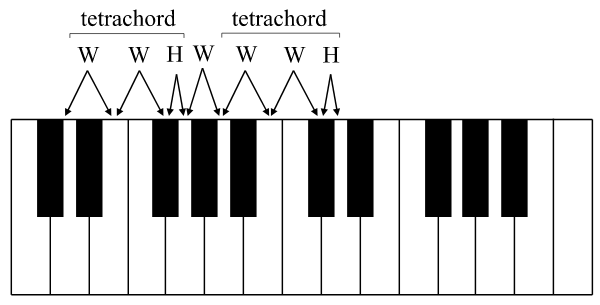
\includegraphics[width=0.6\textwidth]{img/tetrachord}
        \caption{Tetrachords in a (D) major scale}
    \end{center}
\end{figure}

A major scale uses all the 7 notes in order. No one is skipped and there are no duplicates.

\subsection{Key signatures}
There are 15 major key signatures:
\begin{itemize}
    \item 1 with no accidentals: C Major.
    \item 7 with $1$ to $7$ flats.
    \item 7 with $1$ to $7$ sharps.
\end{itemize}

\begin{figure}[h]
    \begin{center}
        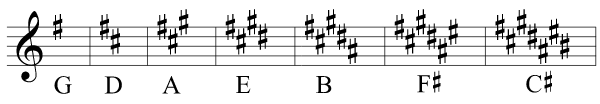
\includegraphics[width=0.8\textwidth]{img/majorsharp}
        \caption{Major key signatures (sharps)}
        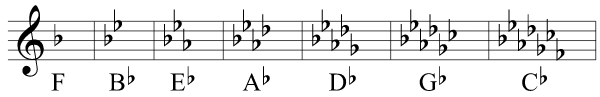
\includegraphics[width=0.8\textwidth]{img/majorflat}
        \caption{Major key signatures (flats)}
    \end{center}
\end{figure}
A key signature can be quickly identified with the following mnemonic:
\begin{itemize}
    \item With \emph{sharps}: +1 half step from the last ``sharped note''.
    \item With \emph{flats}: the second to last flat is the key (along with the flat).
\end{itemize}

\section{Minor scales}
\section{Circle of fifths}
\end{document}